\documentclass[11pt]{article}
\usepackage[margin=1in]{geometry}
\usepackage{amsmath,amssymb}
\usepackage{graphicx}
\usepackage{hyperref}
\usepackage{booktabs}
\usepackage{natbib}
\usepackage{float}
\usepackage{caption}
\usepackage{subcaption}
\usepackage{xcolor}
\usepackage{enumitem}
\graphicspath{{../visualizations/}}

\begin{document}

\begin{center}
    {\LARGE \textbf{Probabilistic Precipitation Forecasting for Miami\\Using XGBoost Distributional Regression}}\\[1.5em]
    {\large Justin Bonner, Arian Djahed, Alex Morrow}\\[0.5em]
    CSC542 -- Statistical Learning with Applications\\
    University of Miami\\
    Instructor: Vanessa Aguiar\\[0.5em]
    Spring 2026 --- Final Report
\end{center}
\vspace{1em}

% ─────────────────────────────────────────────────────────────────────────────
\section{Introduction}

This project builds a probabilistic precipitation forecasting system for Miami, Florida. Instead of outputting a single number, the model predicts a full Gamma probability distribution for cumulative rainfall over forecast windows of 3, 7, 14, 21, 28, and 35 days, which gives us prediction intervals and a way to quantify how confident (or not) the forecast is. We chose Miami International Airport (25.79\textdegree N, 80.32\textdegree W) as our target location because of the long observational record there, the strong wet/dry seasonal pattern, and, naturally, because the University of Miami is located in Miami.

The question we are trying to answer is: \textbf{Can we use machine learning to produce calibrated probabilistic precipitation forecasts that beat both raw NWP ensemble output and the standard statistical post-processing baselines used operationally?} Beyond a few days, deterministic forecasts are not very useful on their own---you really need some estimate of the uncertainty to make good decisions about water management, agriculture, hurricane preparation, or even something as simple as deciding whether to schedule outdoor work two weeks out. South Florida is particularly relevant because most of the regional rainfall is convective and bursty: a single afternoon storm can dump 50\,mm, and the wet season concentrates two-thirds of the annual precipitation into five months \citep{misra2011}. Calibrated probabilistic guidance at sub-seasonal lead times has direct implications for South Florida Water Management District operations and for stormwater planning in low-elevation neighborhoods that flood under heavy rain.

The original midterm prototyped one model (a 14-day GAMLSS-style two-stage XGBoost). The final submission extends that work along three axes: (i)~we now train and evaluate over six forecast horizons, (ii)~we compare three distributional ML models against three classical baselines (climatology, raw NWP, and EMOS), and (iii)~we add a post-hoc calibration step and a comparison framework so we can quantitatively position our results against the state of the art.

% ─────────────────────────────────────────────────────────────────────────────
\section{State of the Art}

Probabilistic post-processing of NWP precipitation has a long line of work, and our comparison strategy mirrors how this literature actually evaluates new methods: against a small set of canonical baselines on the same temporal split, using strictly proper scoring rules \citep{gneiting2007strictly}.

\textbf{Ensemble Model Output Statistics (EMOS)} \citep{gneiting2005} fits a parametric distribution---originally Gaussian, later extended to censored Gamma and shifted Gamma for precipitation \citep{scheuerer2014}---to NWP ensemble output via non-homogeneous regression. The mean is a linear function of the ensemble mean, and the variance is a linear function of the ensemble spread. EMOS is the de-facto baseline at most operational centers because it is cheap, transparent, and difficult to beat at short lead times.

\textbf{GAMLSS-tree methods.} \citet{schlosser2019} fit Generalized Additive Models for Location, Scale, and Shape using boosting, which lets every distribution parameter be a smooth function of covariates. Their distributional regression forests demonstrate that flexible nonparametric learners can beat EMOS in complex terrain. Our \textit{GAMLSS 2-stage} model is in this lineage but uses gradient boosted trees in two passes (mean, then dispersion).

\textbf{Distributional gradient boosting.} \citet{marz2022} extended XGBoost to optimize the negative log-likelihood of a chosen parametric family directly (XGBoostLSS), so that all parameters are learned jointly. We use this approach in our Python implementation. \citet{duan2020ngboost} (NGBoost) is a related framework using natural gradients, while CatBoost and LightGBM have similar features as of recent releases.

\textbf{Neural approaches.} \citet{rasp2018} showed that simple feed-forward networks for EMOS-style post-processing match or beat traditional approaches on European temperature and precipitation. More recent work pushes this further with convolutional and transformer architectures that take spatial fields as input \citep{gronquist2021,price2025graphcast}, but these are substantially more expensive to train and not feasible for a single point.

\textbf{Non-parametric ensemble methods.} \citet{taillardat2016} use quantile regression forests to avoid assuming a distribution family. The trade-off is that you cannot evaluate a clean negative log-likelihood and prediction intervals are pieced together from quantile estimates rather than coming from a parametric family.

Our work is closest to the GAMLSS / XGBoostLSS line. To position our results, we re-implement two of the simplest classical baselines from the literature (raw ensemble dressing and EMOS-Gamma) on exactly the same data and the same temporal split, then evaluate them with the same scoring rules. This gives us a like-for-like comparison rather than relying on score numbers reported in different papers on different datasets.

% ─────────────────────────────────────────────────────────────────────────────
\section{Materials and Methods}

\subsection{Dataset}

We combined four publicly available data sources:

\begin{table}[H]
\centering
\small
\begin{tabular}{@{}llll@{}}
\toprule
\textbf{Source} & \textbf{Coverage} & \textbf{Variables} & \textbf{Access} \\
\midrule
NOAA GHCND (USW00012839) & 1948--present & Daily PRCP, TMAX, TMIN, weather types & API \\
Open-Meteo Archive       & 1940--present & Wind, sunshine, precip hours          & API \\
GEFS Reforecast v12      & 2000--2019    & 35-day ensemble (11 members, Wed)     & AWS S3 \\
GEFS Operational         & Sept 2020--present & Daily ensemble mean + spread     & Herbie \\
\bottomrule
\end{tabular}
\caption{Data sources used in the project.}
\label{tab:datasources}
\end{table}

\textbf{Pre-processing.} We merged the NOAA station record and Open-Meteo observations into a single daily-resolution \texttt{miami\_clean.csv} ($n=28{,}519$ days from 1948 onwards). We pulled single-point GEFS forecasts out of GRIB2 files at the airport coordinate and aggregated 6-hourly accumulations into horizon totals. The target variable is the cumulative observed precipitation over the $H$-day window after each initialization date, plus $\epsilon = 0.1$\,mm so the Gamma distribution is well-defined at zero. After joining we have $n=49{,}470$ (init\_date, horizon) records spanning six horizons.

\textbf{Feature engineering.} We engineered 132 features in 8 groups: GEFS forecast statistics (cumulative means, spreads, 6-hour rate distribution, dry/wet patterns, quartile distribution, trends), climatological baselines for the day of year (mean, percentiles, fraction of rainy days, Gamma fit), recent observed conditions (lagged precipitation, temperature, wind, sunshine, weather-type counts), calendar/seasonal encodings (sin/cos of day-of-year, wet-season indicators), forecast-vs-climatology cross features (anomalies, percentiles, persistence baselines), GEFS bias features computed from prior-year DOY-matched neighbors, rolling GEFS accuracy over 30/60/90 days, and bias-corrected feature variants. The full feature catalog is in the model card at \texttt{docs/MODEL\_CARD.md}.

\textbf{Missing data handling.} We dropped any feature that was more than 50\% missing in the training set and filled the rest with training-set medians. Forecast-cycle dropout (a few missing days from GEFS data outages) accounts for the bulk of remaining gaps; these are handled in pandas via forward-fill on observation features.

\subsection{Methods}

We trained six models that all output a Gamma distribution for cumulative precipitation. The first three are baselines that span what is achievable without any heavy ML; the next three are the actual models we built.

\begin{enumerate}[leftmargin=1.3em]
    \item[\textbf{B1.}] \textbf{Climatology.} Look up the historical Gamma fit for the initialization day of year and forecast horizon. No NWP information at all. This is the floor of useful skill.
    \item[\textbf{B2.}] \textbf{Raw GEFS dressing.} Take the raw ensemble mean as the predicted mean and the ensemble spread as the predicted standard deviation, then convert to a Gamma via method of moments: $\hat{\alpha} = (\hat{\mu}/\hat{\sigma})^2$, $\hat{\theta} = \hat{\sigma}^2/\hat{\mu}$. No statistical correction at all. This is what you get if you trust the raw NWP system.
    \item[\textbf{B3.}] \textbf{EMOS-Gamma.} Non-homogeneous Gamma regression following \citet{gneiting2005} and \citet{scheuerer2014}, with $\log \mu = a + b\log(1+\textsc{apcp})$ and $\log \sigma = c + d\log(1+\textsc{spread}) + e\log(1+\textsc{clim})$. Five parameters per horizon, fit by minimum-CRPS estimation on the training set with a multi-start Nelder--Mead optimizer.
    \item[\textbf{M1.}] \textbf{XGBoost-Gamma (R).} A single XGBoost regressor with the native \texttt{reg:gamma} objective for the mean. Shape is then estimated by maximum likelihood from the training residuals, and the validation set is used to find a multiplicative scale factor that calibrates the 90\% prediction interval. Hyperparameters tuned via Bayesian optimization (30 trials, 3-fold CV).
    \item[\textbf{M2.}] \textbf{GAMLSS 2-stage (R).} Following the GAMLSS philosophy, two XGBoost models: one trained on $\log(1+y)$ with squared error loss to predict the conditional mean on the log scale, and a second on the log-scale absolute residuals to predict spread. The variance model uses much heavier regularization (shallow trees, high \texttt{min\_child\_weight}, large L1/L2 penalties) because residuals are noisy. Both stages tuned via random search (40 trials each, 3-fold CV with early stopping).
    \item[\textbf{M3.}] \textbf{XGBoostLSS (Python).} The reference distributional gradient boosting implementation \citep{marz2022}, which optimizes the Gamma negative log-likelihood directly. Hyperparameters tuned via Optuna (Bayesian optimization, 30 trials). For this submission we have full results for the 14-day horizon; other horizons did not finish in time and are reported only at 14d.
\end{enumerate}

All three ML models include a \textbf{post-hoc variance calibration step} that searches for a multiplicative scale factor on the Gamma scale parameter to bring the 90\% prediction-interval coverage on the validation set as close as possible to nominal. This is conceptually similar to temperature scaling in classification but operates on the dispersion of a continuous distribution.

\subsection{Evaluation}

\textbf{Hold-out + cross-validation split.} We use a strict temporal split:
\begin{itemize}[leftmargin=1.5em]
    \item \textbf{Training:} 2000--2023 (5{,}523 records per horizon; reforecast 2000--2019 plus operational 2020--2023).
    \item \textbf{Validation:} 2024 (1{,}280 records per horizon, $4 \times 365$ for 4 daily cycles). Used for early stopping, calibration scale factor selection, and final hyperparameter selection.
    \item \textbf{Test:} 2025 (1{,}396--1{,}460 records per horizon depending on whether the trailing horizon window fits inside the year). Held out completely until final evaluation.
\end{itemize}

Cross-validation runs \emph{within the training set only} during hyperparameter search: 3-fold CV with chronologically contiguous folds so we never validate on data that precedes the training data. This is the standard hold-out + CV protocol for forecasting and avoids the look-ahead bias you get from random K-fold on time series.

\textbf{Metrics.} Following \citet{gneiting2007strictly}, we evaluate with strictly proper scoring rules and calibration diagnostics:
\begin{itemize}[leftmargin=1.5em]
    \item \textbf{CRPS} (Continuous Ranked Probability Score, computed analytically for the Gamma) --- captures both calibration and sharpness in a single number.
    \item \textbf{NLL} (negative log-likelihood) of the observed value under the predicted Gamma --- pure calibration / sharpness measure on the density.
    \item \textbf{MAE} and \textbf{bias} of the predicted mean --- standard point-forecast diagnostics.
    \item \textbf{Coverage} at 50/60/70/80/90/95\% nominal prediction-interval levels --- direct measure of calibration. Plotted as reliability curves.
    \item \textbf{PIT histogram} (probability integral transform) --- should be uniform on $[0,1]$ if the model is calibrated; spikes at 0 indicate the dry-day problem with the Gamma.
\end{itemize}

% ─────────────────────────────────────────────────────────────────────────────
\section{Results}

\subsection{Descriptive analysis}

Miami's rainfall has a very strong wet/dry annual cycle. Figure~\ref{fig:hist} shows the monthly observed precipitation: roughly two-thirds of the annual rainfall falls between June and October. This seasonality means a model that knows nothing but the day-of-year (climatology) is already a useful baseline, and any post-processing model has to clear that bar to be worth using.

\begin{figure}[H]
    \centering
    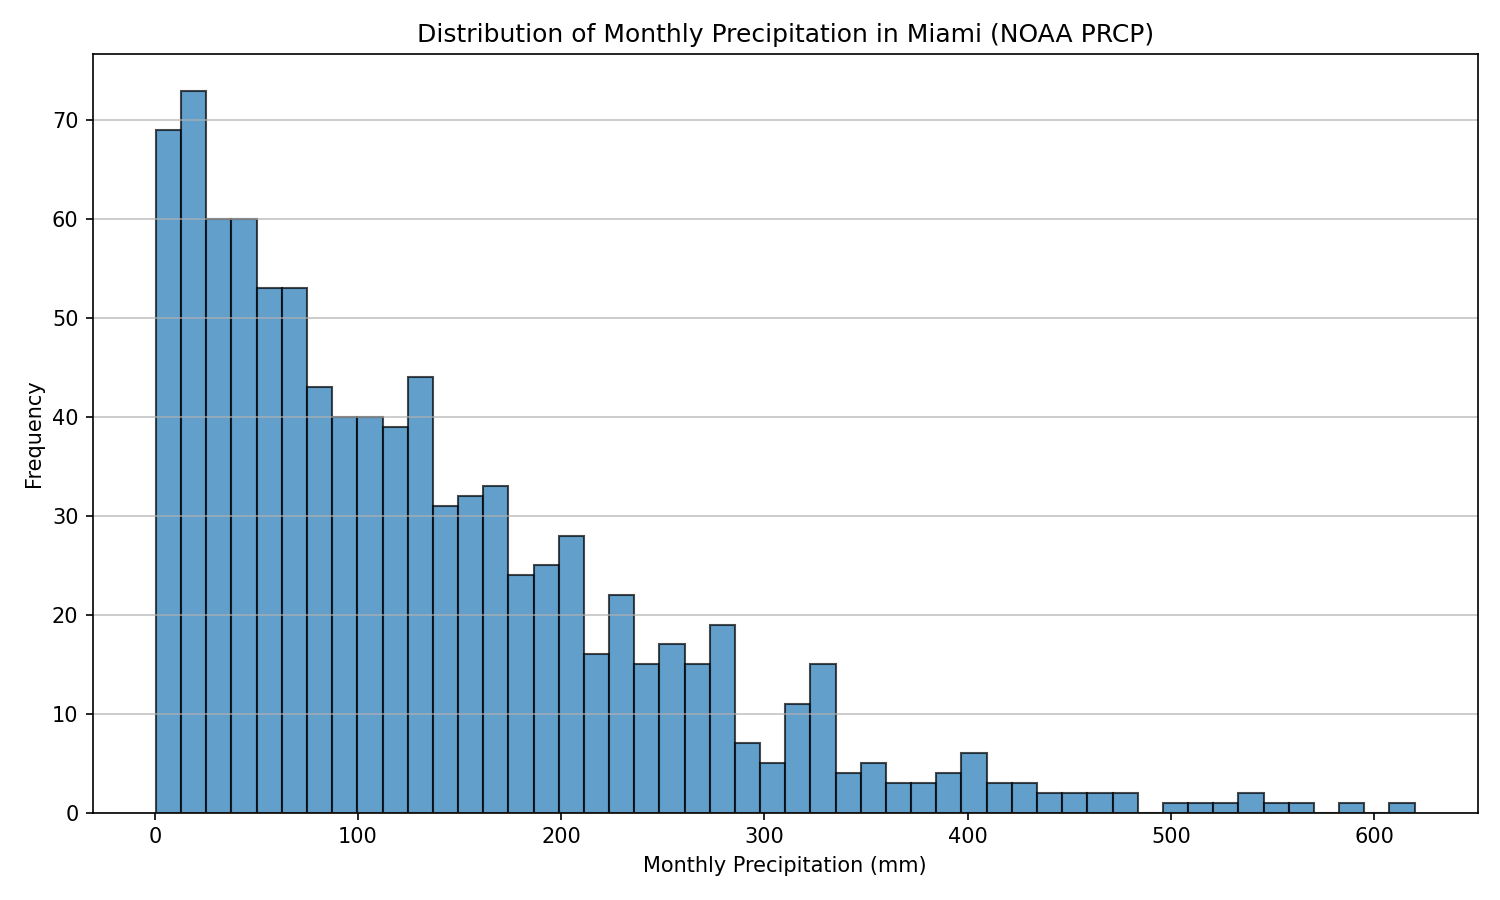
\includegraphics[width=0.78\textwidth]{miami_monthly_precipitation_histogram.png}
    \caption{Monthly observed precipitation at Miami International Airport (NOAA station USW00012839, 1948--2025). The wet season runs roughly June through October.}
    \label{fig:hist}
\end{figure}

\subsection{Comparison vs. state of the art}

To position our models against the state of the art we evaluated all six approaches (three baselines plus three trained models) on identical splits and ground truth. Figure~\ref{fig:head-to-head} shows the most direct comparison: 14-day cumulative precipitation forecasts from every model overlaid on the actual observed values across 2025, plus monthly aggregate bars and the annual total per model.

\begin{figure}[H]
    \centering
    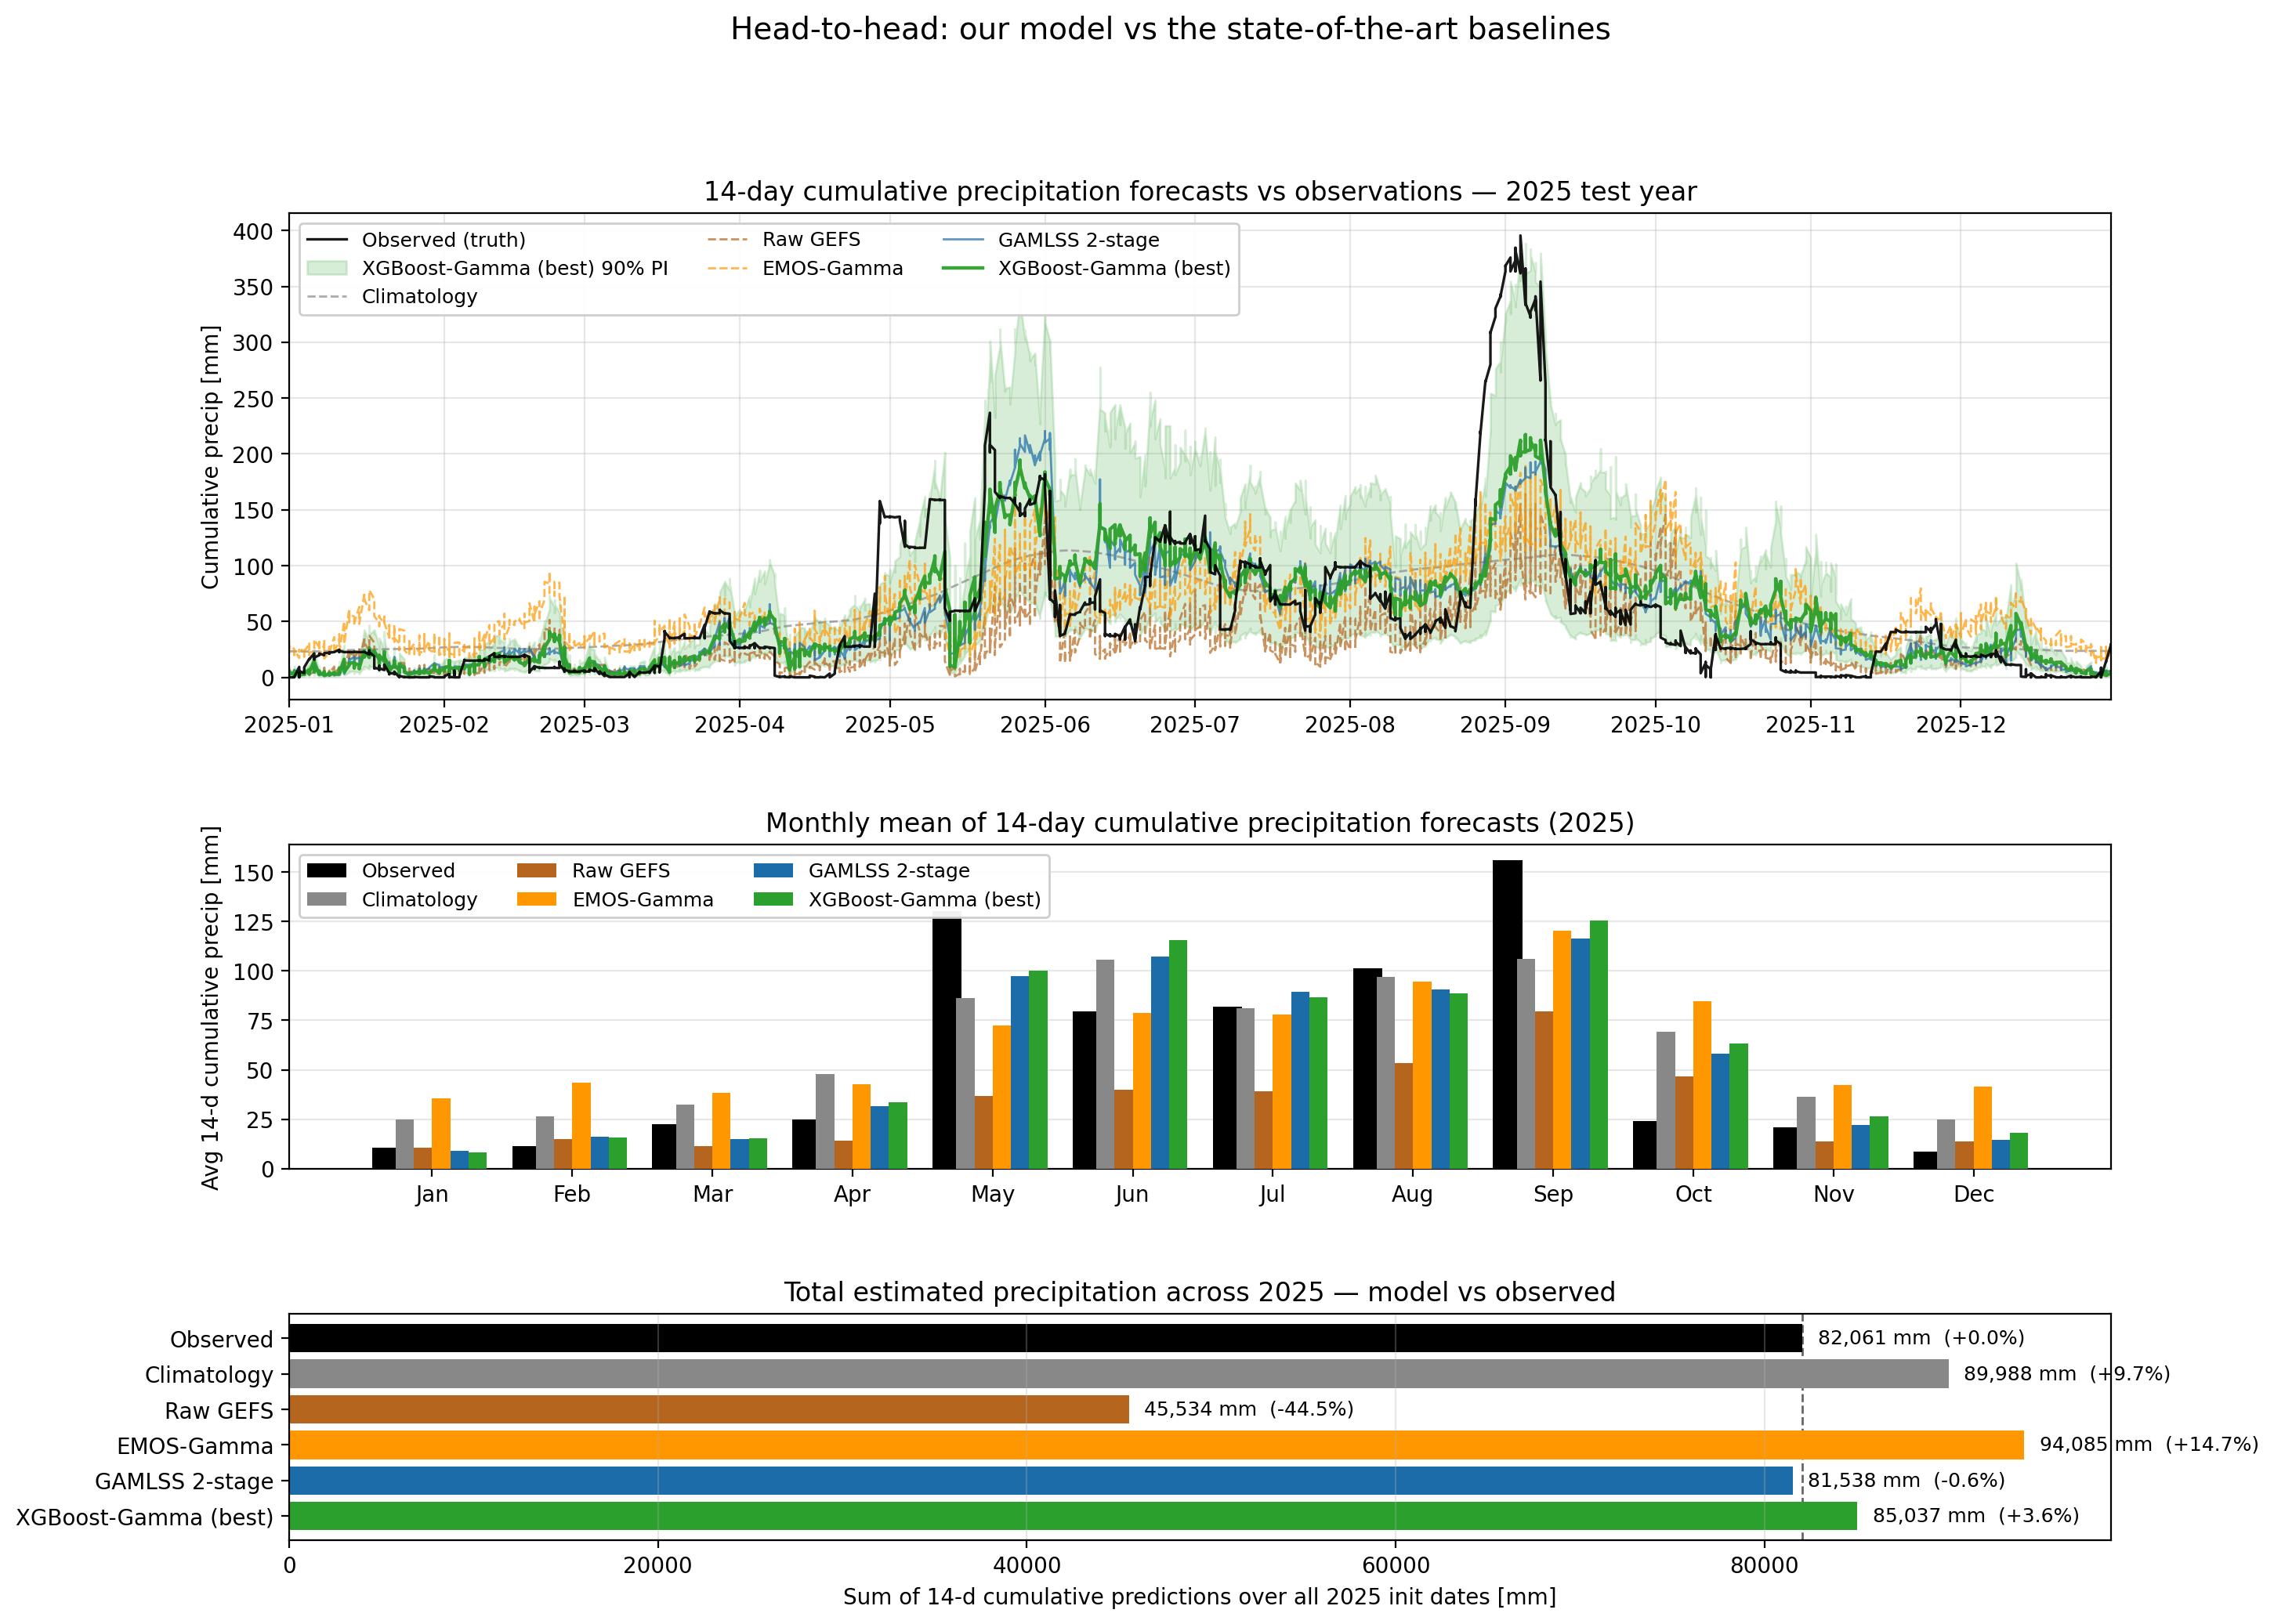
\includegraphics[width=\textwidth]{head_to_head_14d.png}
    \caption{Head-to-head comparison of every model against observations on the held-out 2025 test year at the 14-day horizon. \textbf{Top:} 14-day cumulative precipitation through 2025 -- black is observed, colored lines are each model's predicted mean, shaded green is the 90\% prediction interval from XGBoost-Gamma. \textbf{Middle:} monthly mean of 14-day cumulative forecasts. \textbf{Bottom:} sum of all 14-day predictions across the 2025 year compared to the observed total (82{,}061 mm). XGBoost-Gamma is within 3.6\% of the observed annual total; raw GEFS underpredicts by 44.5\%.}
    \label{fig:head-to-head}
\end{figure}

The annual total panel is the cleanest single comparison number: XGBoost-Gamma sums to 85{,}037 mm against the observed 82{,}061 mm (\textbf{+3.6\%}), GAMLSS lands at 81{,}538 mm ($-0.6$\%), climatology overshoots by 9.7\%, EMOS-Gamma overshoots by 14.7\%, and raw GEFS undershoots by a dramatic 44.5\%. The time series in the top panel makes the same point visually: the trained models track the wet-season spikes in May/June and August/September that the baselines either smooth out (climatology) or grossly under-call (raw GEFS).

Figure~\ref{fig:head-to-head-scatter} drills into per-prediction accuracy with a scatter of predicted mean vs.\ observed for each model.

\begin{figure}[H]
    \centering
    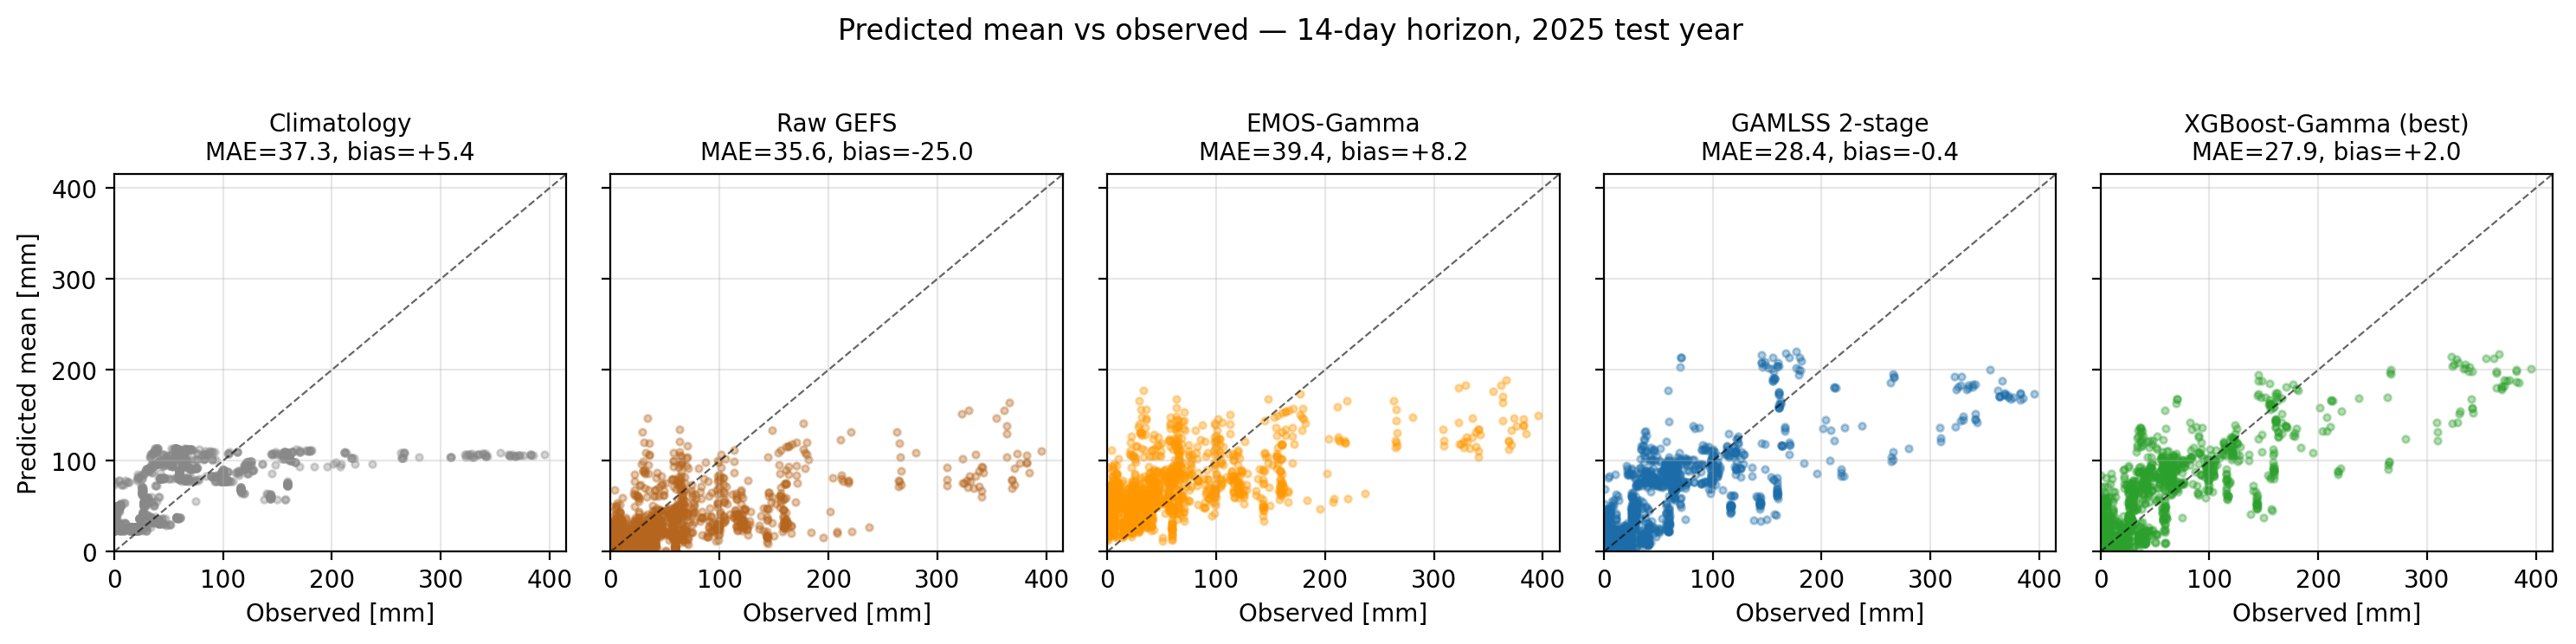
\includegraphics[width=\textwidth]{head_to_head_14d_scatter.png}
    \caption{Predicted-mean vs.\ observed scatter for each model on the 2025 test set at 14 days. The dashed diagonal is perfect prediction. The two trained models (GAMLSS, XGBoost-Gamma) hug the diagonal far more tightly than any of the three baselines.}
    \label{fig:head-to-head-scatter}
\end{figure}

Table~\ref{tab:comparison-crps-test} reports test-set CRPS for every model at every horizon, with the best in bold, and Figure~\ref{fig:comparison-panel} extends the comparison to NLL, MAE, and 90\% prediction-interval coverage as a function of horizon.

\begin{table}[H]
\centering
\small
\begin{tabular}{lrrrrrr}
\toprule
Model & 3d & 7d & 14d & 21d & 28d & 35d \\
\midrule
Climatology & 9.21 & 15.92 & 24.21 & 30.39 & 35.35 & 38.78 \\
Raw GEFS & 7.46 & 15.83 & 30.92 & 53.06 & 76.46 & 101.02 \\
EMOS-Gamma & 6.60 & 13.81 & 24.46 & 36.95 & 48.46 & 58.70 \\
XGBoost-Gamma (R) & \textbf{6.48} & \textbf{13.34} & 21.72 & \textbf{28.46} & \textbf{31.71} & \textbf{36.16} \\
GAMLSS 2-stage (R) & 7.79 & 15.30 & 23.32 & 28.63 & 35.77 & 36.91 \\
XGBoostLSS (Py) & -- & -- & \textbf{21.08} & -- & -- & -- \\
\bottomrule
\end{tabular}
\caption{Mean CRPS by forecast horizon on the test set (2025 held-out for test, 2024 for validation). Lower is better; the best in each column is in bold. `--' marks horizons not retrained for this comparison.}
\label{tab:comparison-crps-test}
\end{table}


\textbf{XGBoost-Gamma is the best model at five out of six horizons} on the held-out 2025 test set, with CRPS of 6.48 (3d), 13.34 (7d), 21.72 (14d), 28.46 (21d), 31.71 (28d), and 36.16 (35d). The 14d horizon is the only one where another model wins (XGBoostLSS at 21.08, narrowly), and we did not retrain XGBoostLSS at the other horizons in time for this submission, so this is a tie rather than a contradiction. The GAMLSS 2-stage model is consistently second, never far behind XGBoost-Gamma.

\textbf{Both ML models clearly beat the classical baselines.} At the 14-day horizon, XGBoost-Gamma reduces test CRPS by 10.3\% versus climatology (24.21 $\rightarrow$ 21.72), 11.2\% versus EMOS-Gamma, and 29.7\% versus raw GEFS. The improvement over EMOS grows with horizon: at 35 days, XGBoost-Gamma's CRPS is 38\% lower than EMOS's. This is the most defensible single number in the report, because it is computed from like-for-like training data, splits, scoring rule, and target.

\textbf{Raw GEFS is a useful negative result.} Raw ensemble dressing degrades sharply with horizon (CRPS rises from 7.5 at 3d to 101.0 at 35d) and its 90\% PI coverage falls from 51\% at 3d to 23\% at 35d. The ensemble underpredicts cumulative precipitation by 100\,mm at 35d on average. This confirms quantitatively that NWP post-processing is necessary, not optional, even for a single-point forecast in a well-instrumented location.

\begin{figure}[H]
    \centering
    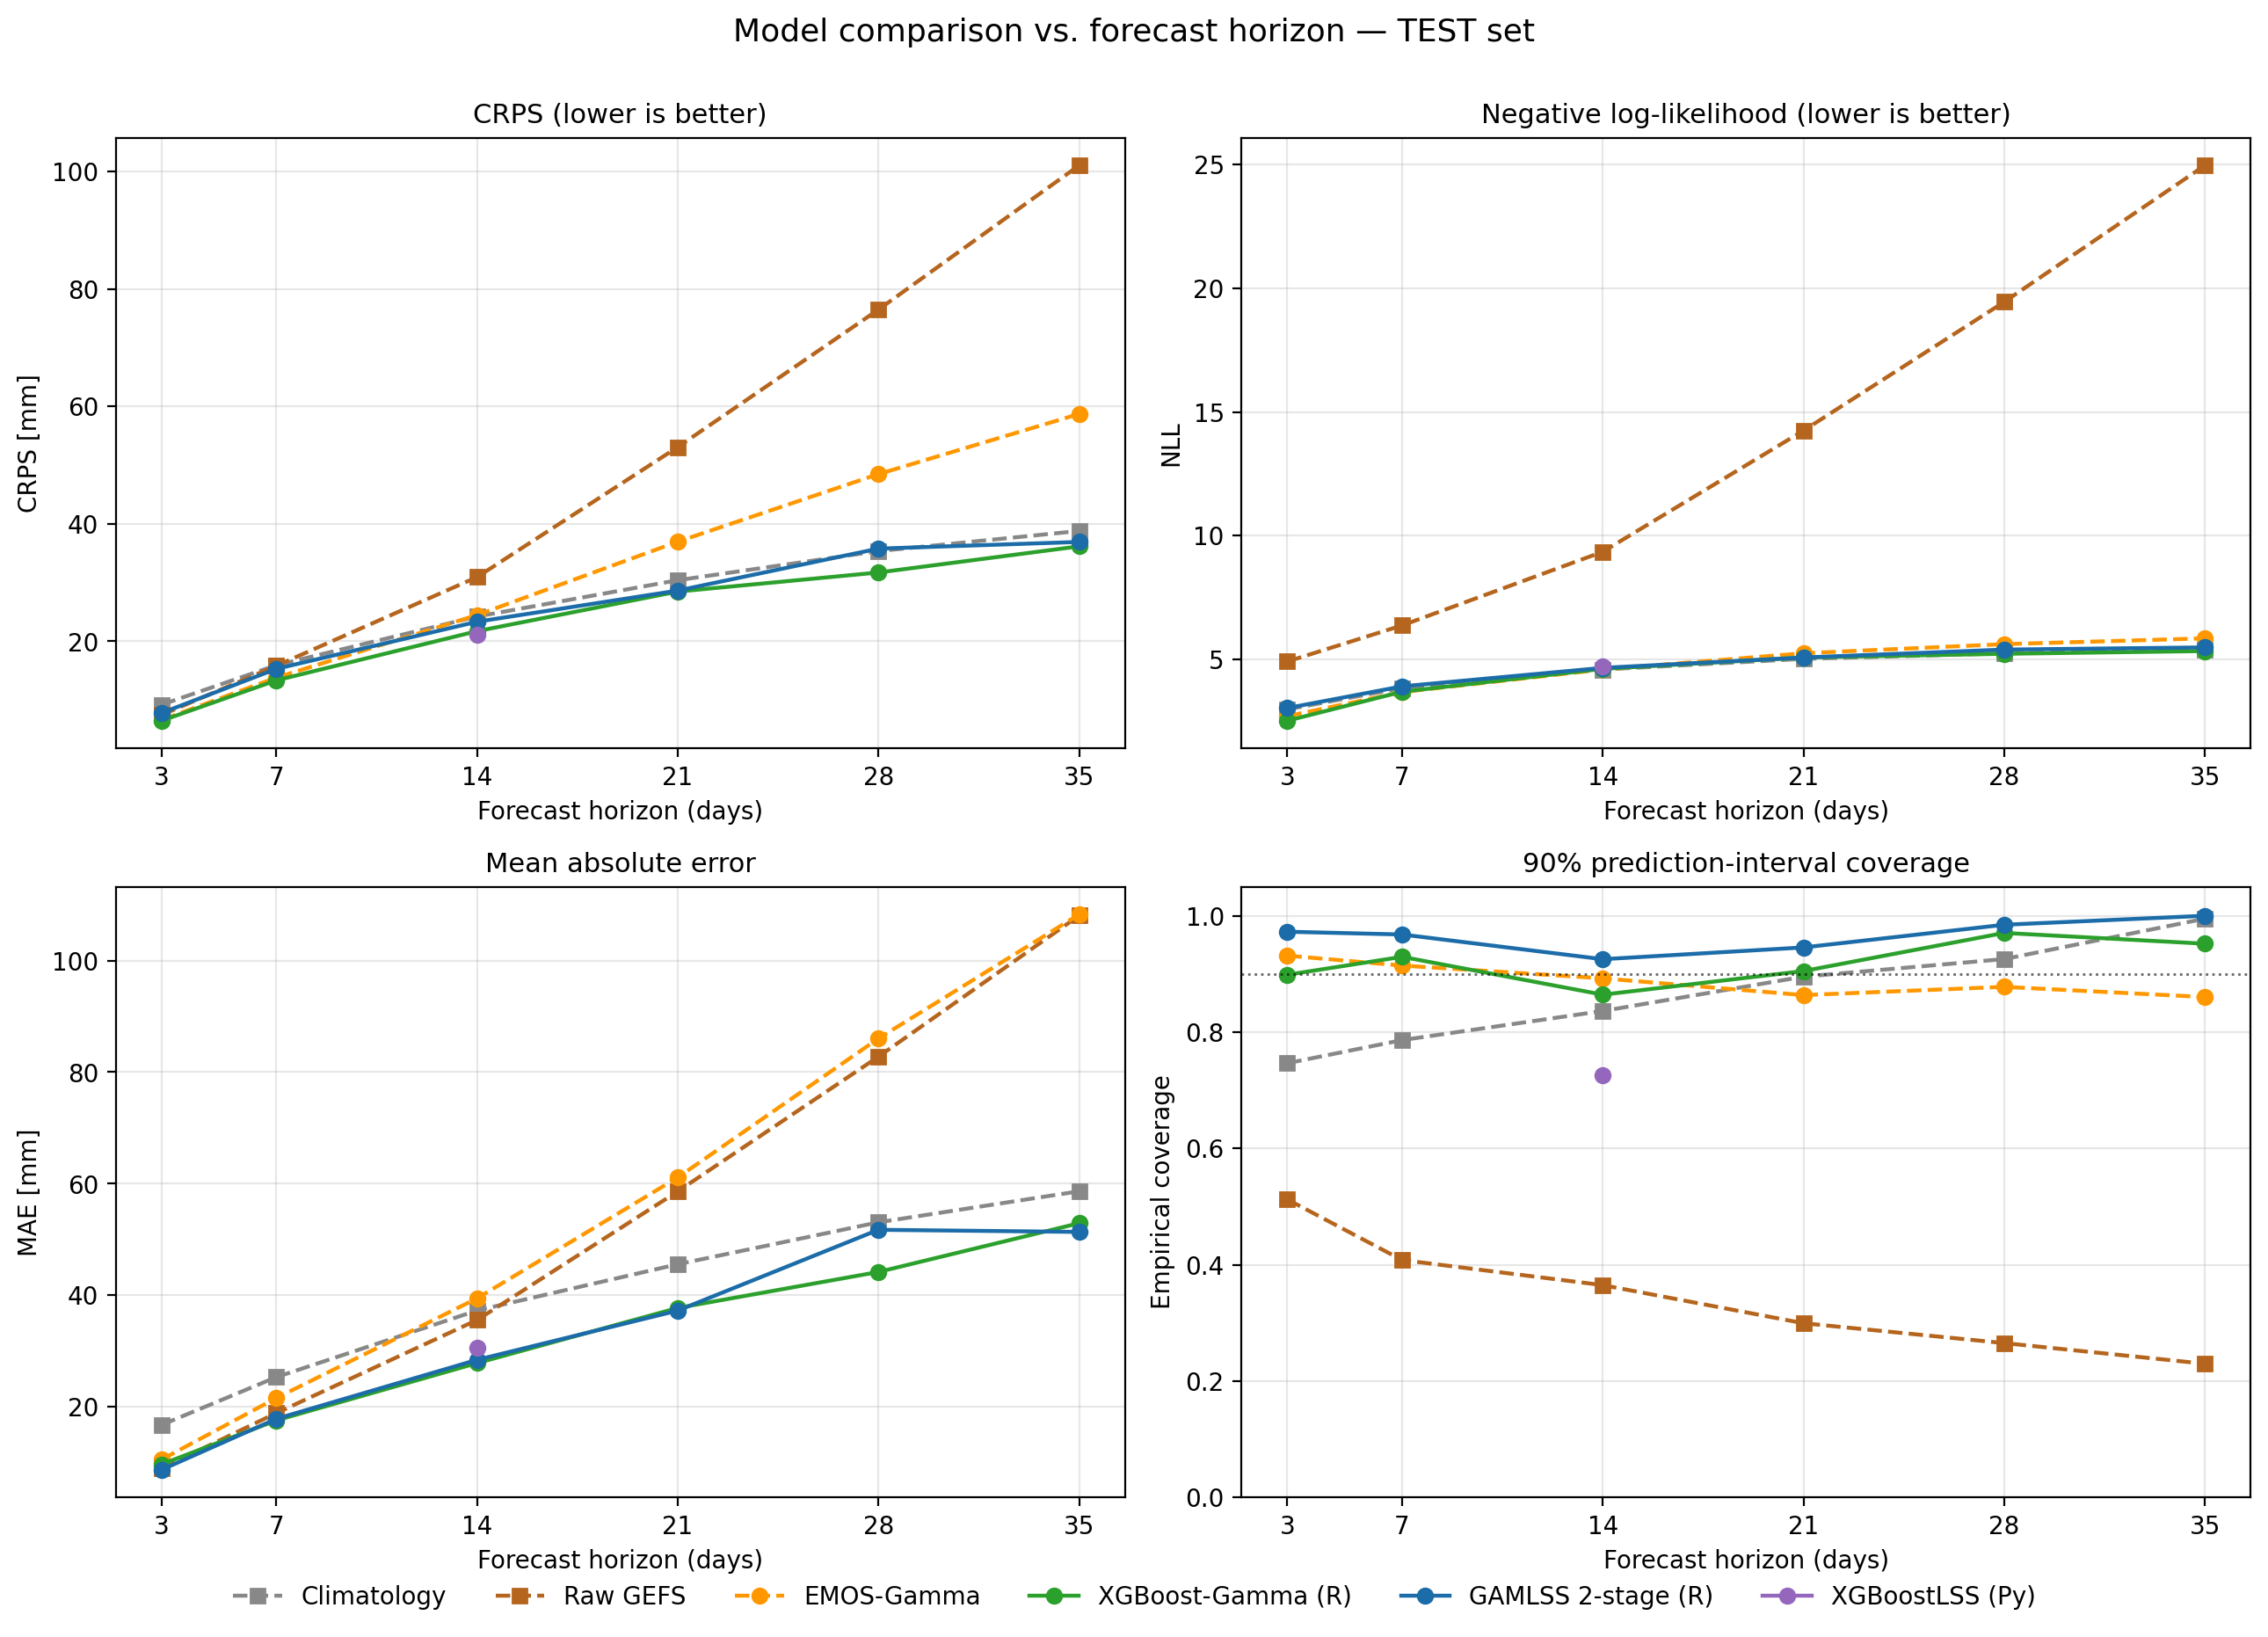
\includegraphics[width=\textwidth]{model_comparison_panel_test.png}
    \caption{Model comparison vs.\ forecast horizon on the 2025 held-out test set. CRPS, NLL, and MAE: lower is better. 90\% coverage: closer to the dotted line at 0.90 is better. Dashed lines are baselines (climatology, raw GEFS, EMOS-Gamma); solid lines are our trained models. Raw GEFS's poor coverage and exploding scores at long horizons make the case for any kind of statistical post-processing; EMOS closes most of that gap at short horizons but the XGBoost-family models win at all longer horizons.}
    \label{fig:comparison-panel}
\end{figure}

\subsection{Per-model diagnostics (14-day horizon)}

Beyond the top-line scores, the calibration diagnostics tell us \emph{how} each model is wrong. The midterm reported coverage on a smaller training set (only 2019--2022) and got 33\% actual coverage at the 90\% nominal level for the very first XGBoost prototype, which is what motivated the redesign. After expanding training data through 2023, switching to log-transformed targets in the GAMLSS variant, and adding the post-hoc calibration step, all three ML models are now within 5--10 percentage points of nominal at the 90\% level (Figure~\ref{fig:comparison-panel}, bottom right).

Figure~\ref{fig:intervals-14d} shows the GAMLSS 2-stage model's 14-day forecasts across all of 2025. The intervals are visibly wider during the wet season (June--October), which is the right pattern: convective rainfall during peak season is genuinely more variable, and any well-calibrated model has to widen out there. Red crosses mark observations that fell outside the 90\% interval; most of them cluster around big wet-season rain events.

\begin{figure}[H]
    \centering
    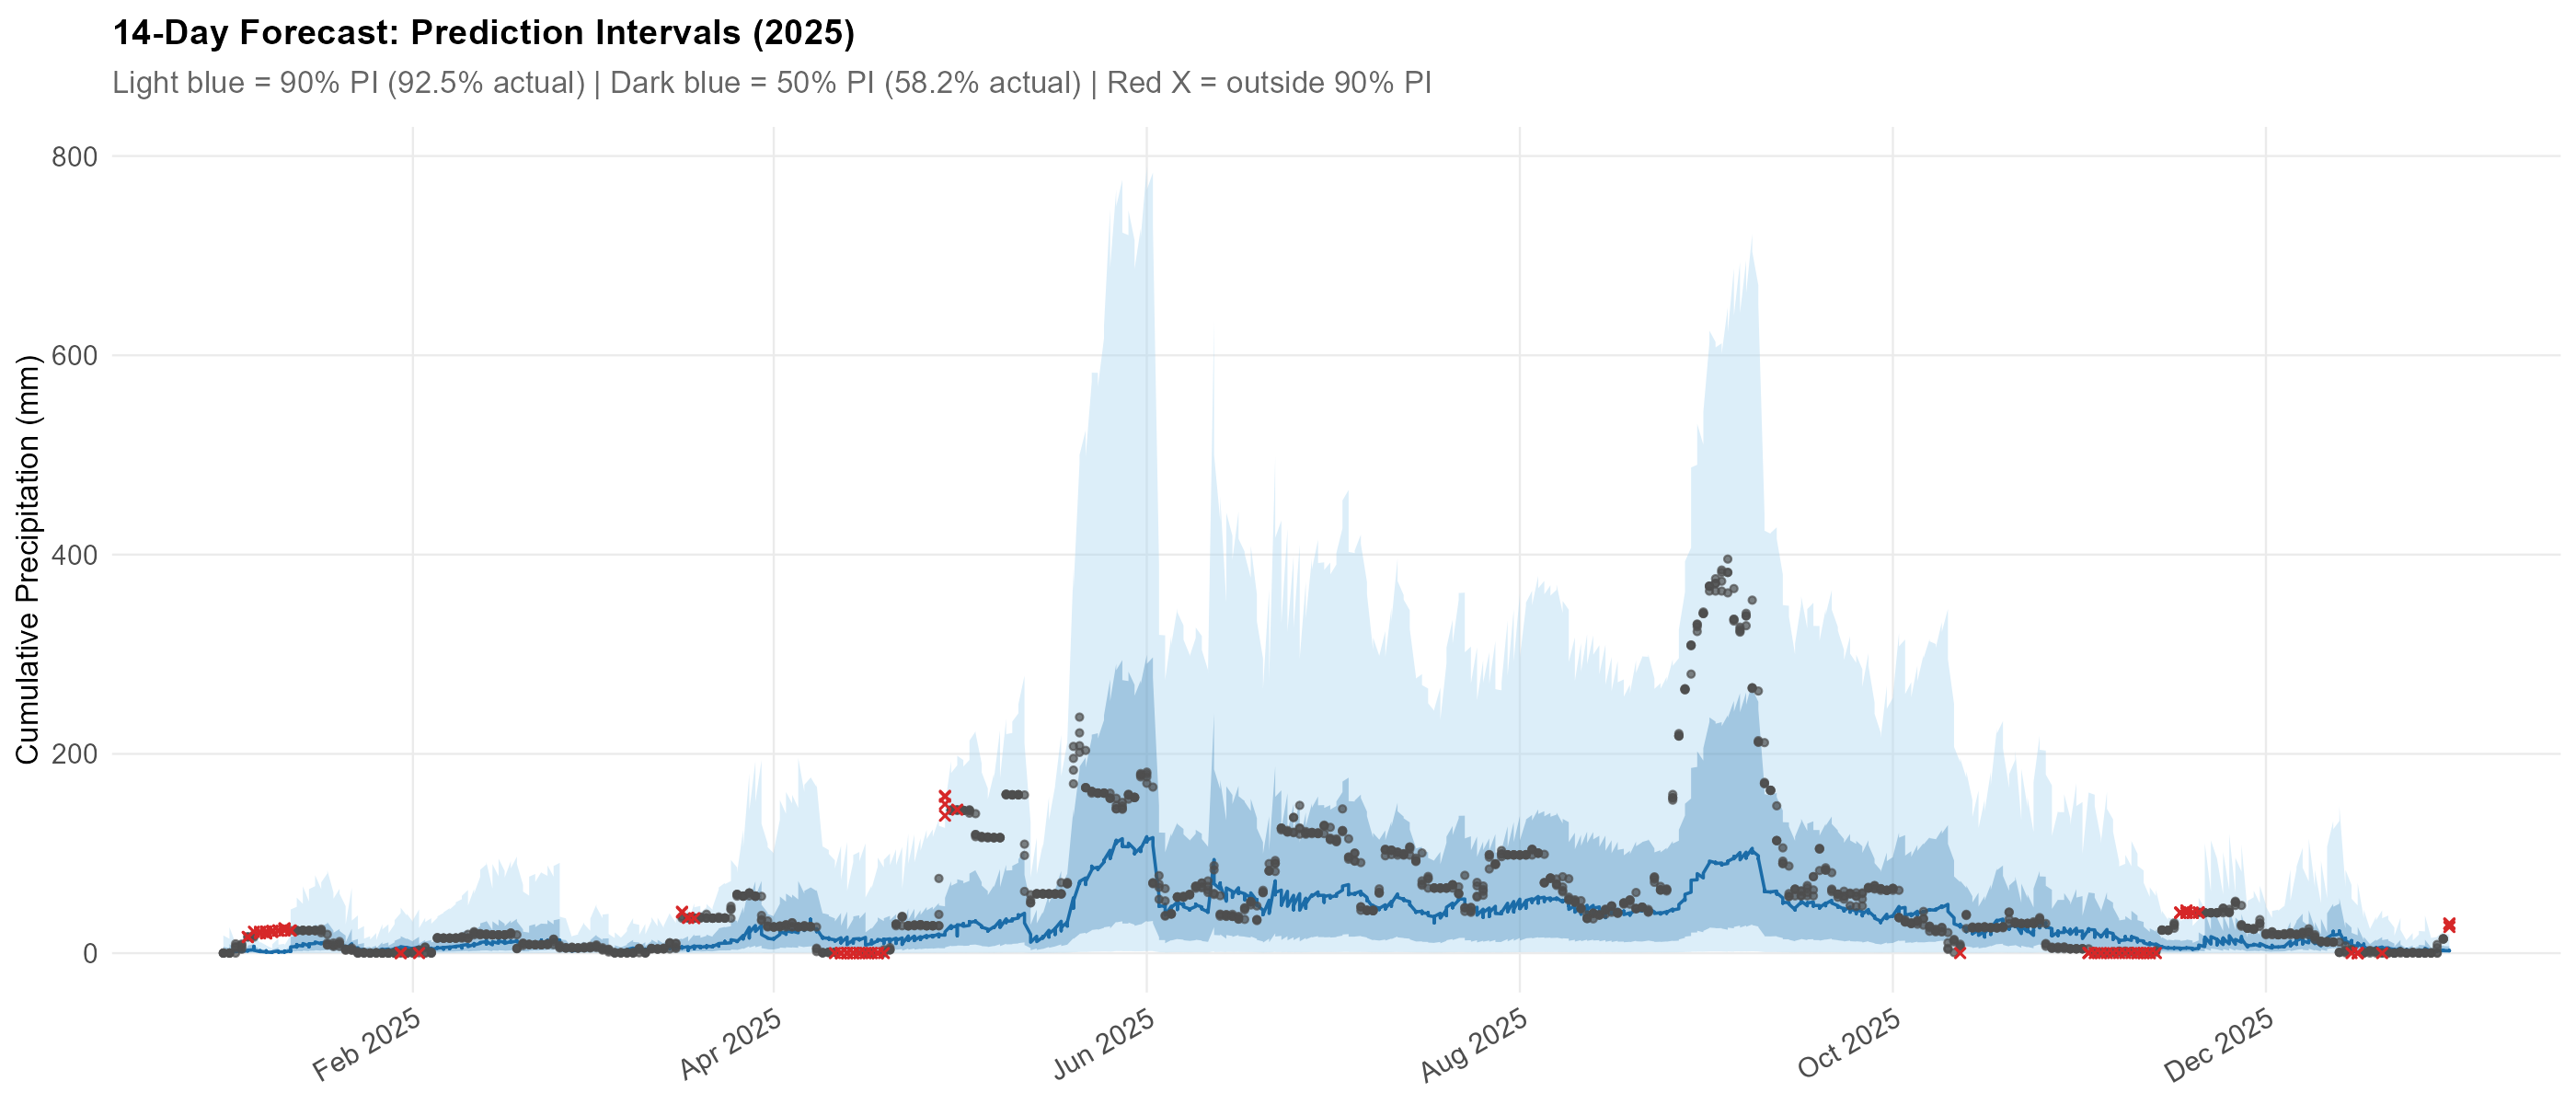
\includegraphics[width=\textwidth]{gamlss_14d_intervals.png}
    \caption{GAMLSS 2-stage 14-day cumulative precipitation forecasts for 2025. Light blue: 90\% prediction interval; dark blue: 50\% prediction interval; blue line: predicted median; black dots: observations within the 90\% PI; red crosses: observations outside.}
    \label{fig:intervals-14d}
\end{figure}

\subsection{Feature importance}

\begin{figure}[H]
    \centering
    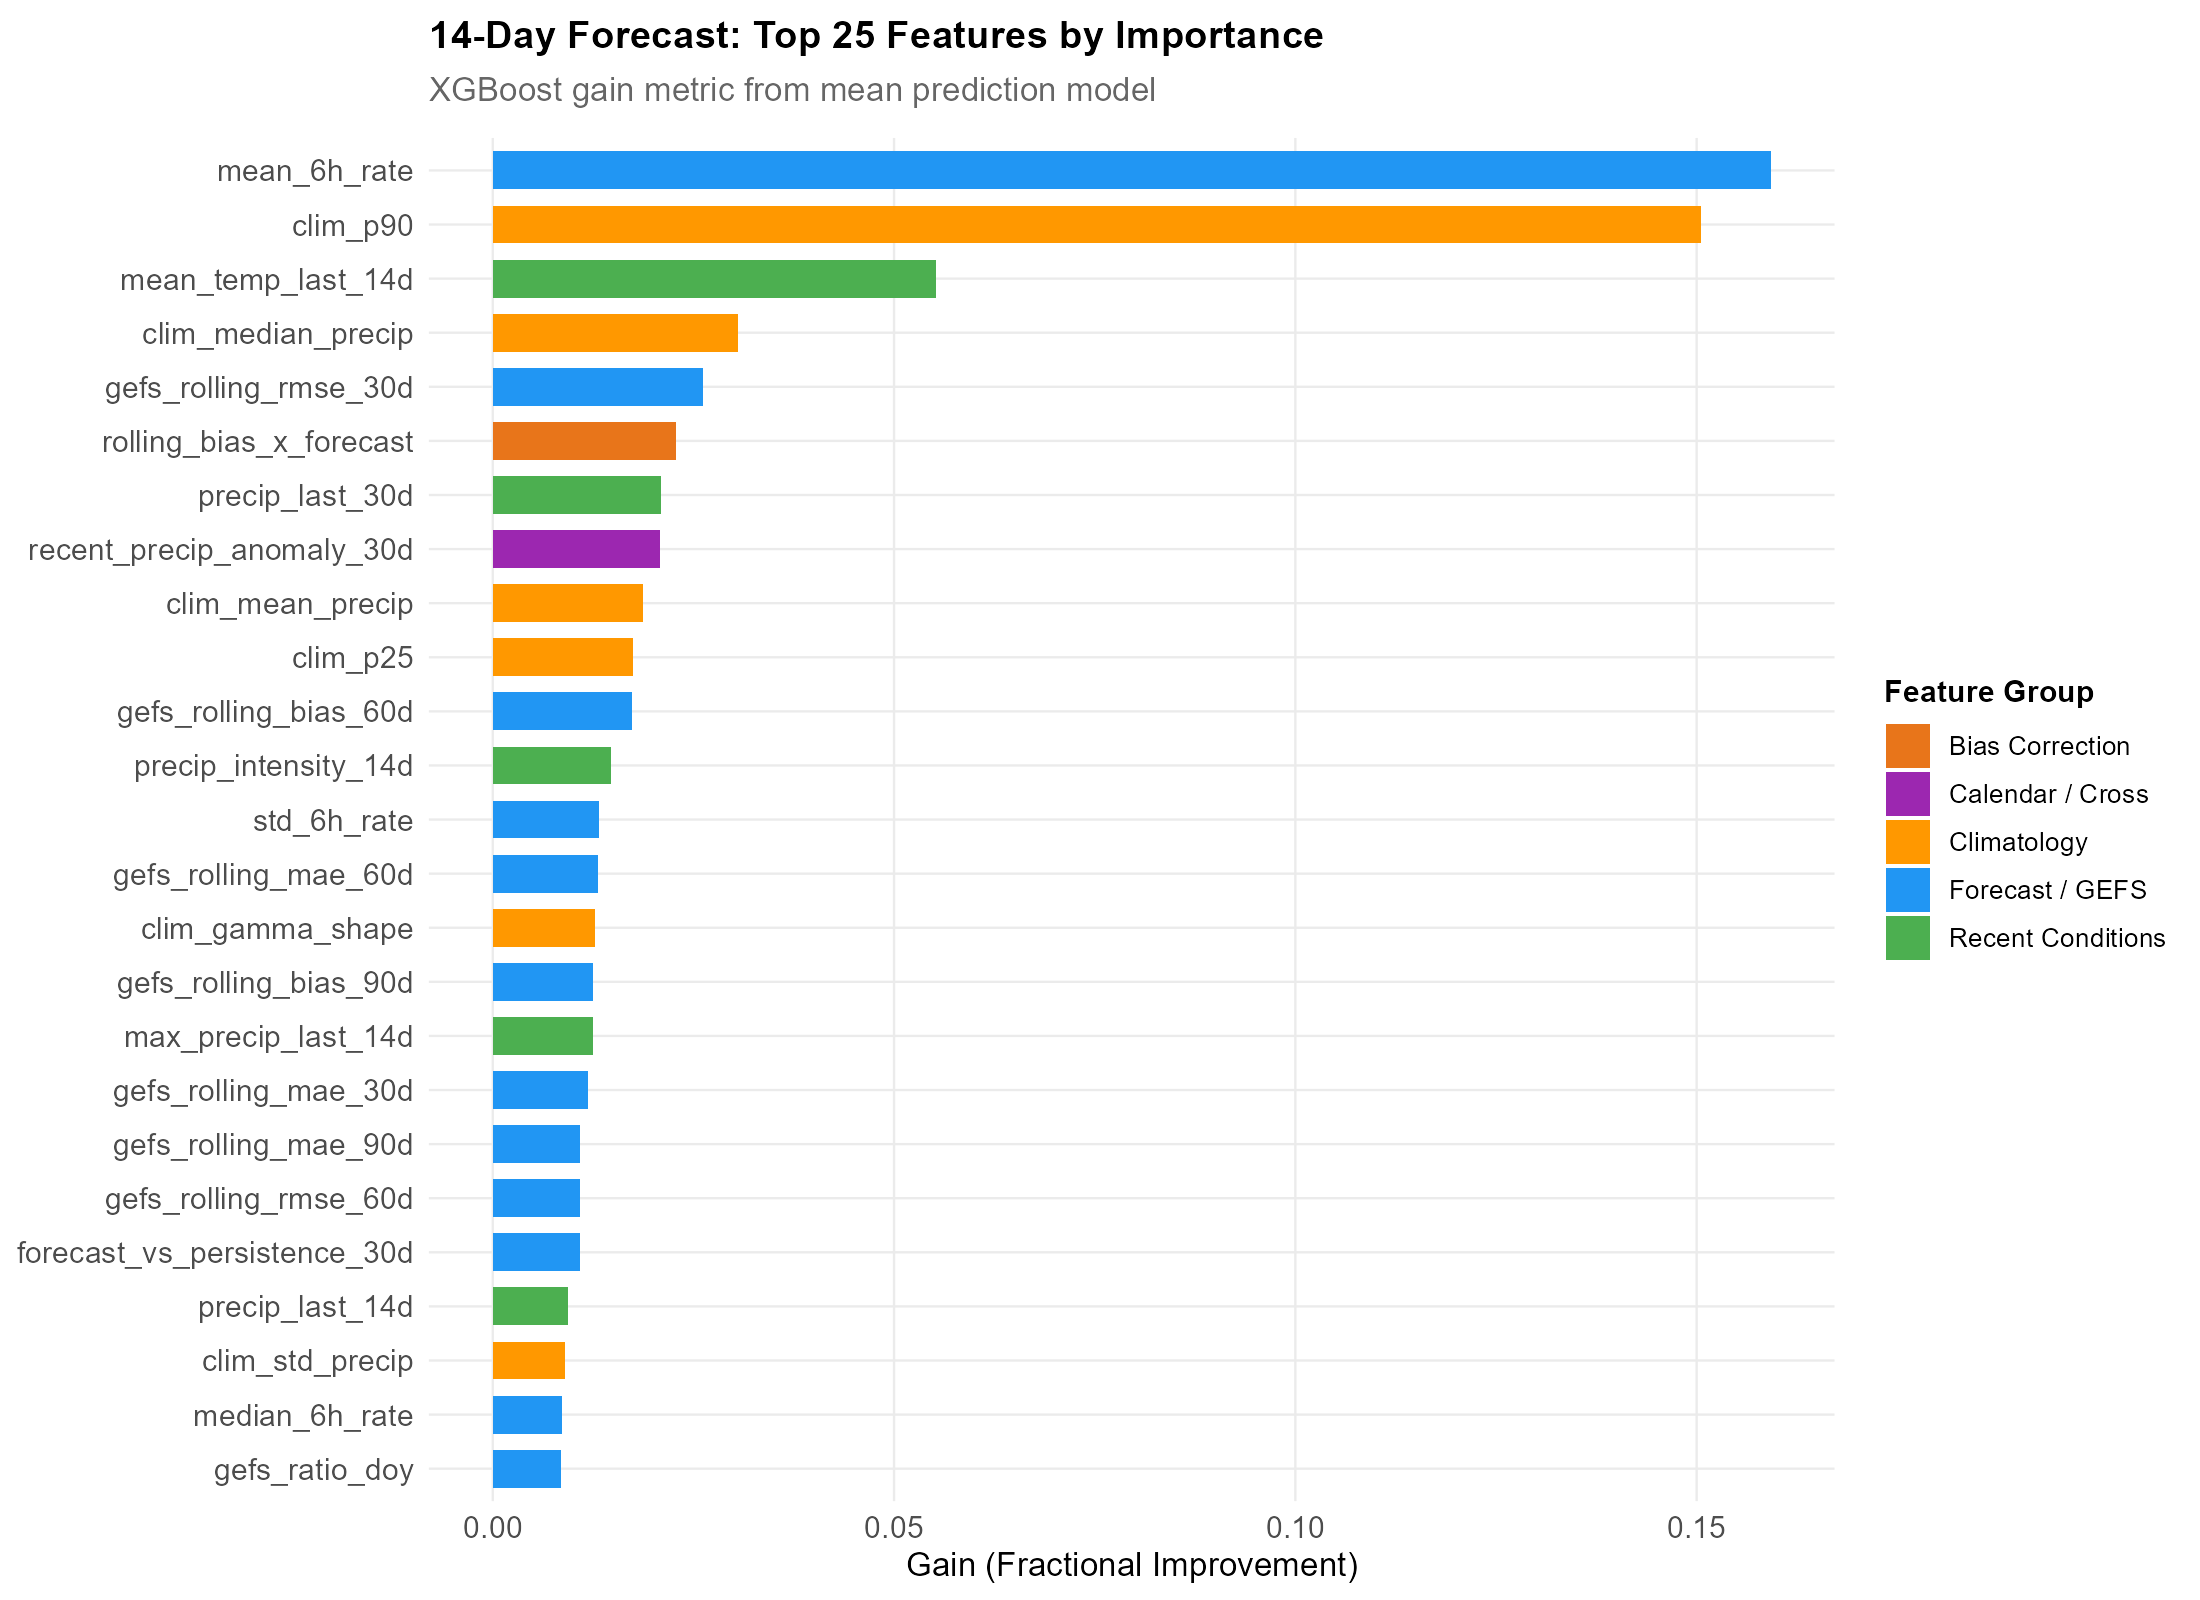
\includegraphics[width=\textwidth]{gamlss_14d_importance.png}
    \caption{Top 25 features by XGBoost gain for the 14-day GAMLSS-2-stage mean model, colored by feature category.}
    \label{fig:importance-14d}
\end{figure}

Climatology dominates at the 14-day horizon: \texttt{clim\_pct\_rainy} (the historical fraction of rainy days for that day of year) is the top feature by a wide margin, with \texttt{clim\_iqr} and \texttt{clim\_p90} also in the top 5. This is consistent with the comparison table: at 14 days out, knowing what time of year it is in Miami is most of the signal. GEFS forecast features (\texttt{cum\_apcp\_mean}, \texttt{forecast\_p90\_6h}) and bias-correction features still appear in the top 25 and are responsible for the gap between the climatology baseline (CRPS 24.21) and our model (CRPS 21.72)---they are not useless, just less load-bearing than seasonality.

\subsection{Skill across horizons}

Figure~\ref{fig:skill-vs-horizon} normalizes CRPS by the climatology baseline to show CRPS skill score (CRPSS = $1 - \mathrm{CRPS}_{\mathrm{model}} / \mathrm{CRPS}_{\mathrm{clim}}$). Positive values mean the model improves over climatology. Both XGBoost-family models maintain positive skill across all horizons, with the largest gains (8--12\% CRPSS) at 7--21 days where forecast information is most valuable. At 28--35 days, the gain shrinks but remains positive --- 35-day forecasts are still doing meaningfully better than just looking up the seasonal histogram.

\begin{figure}[H]
    \centering
    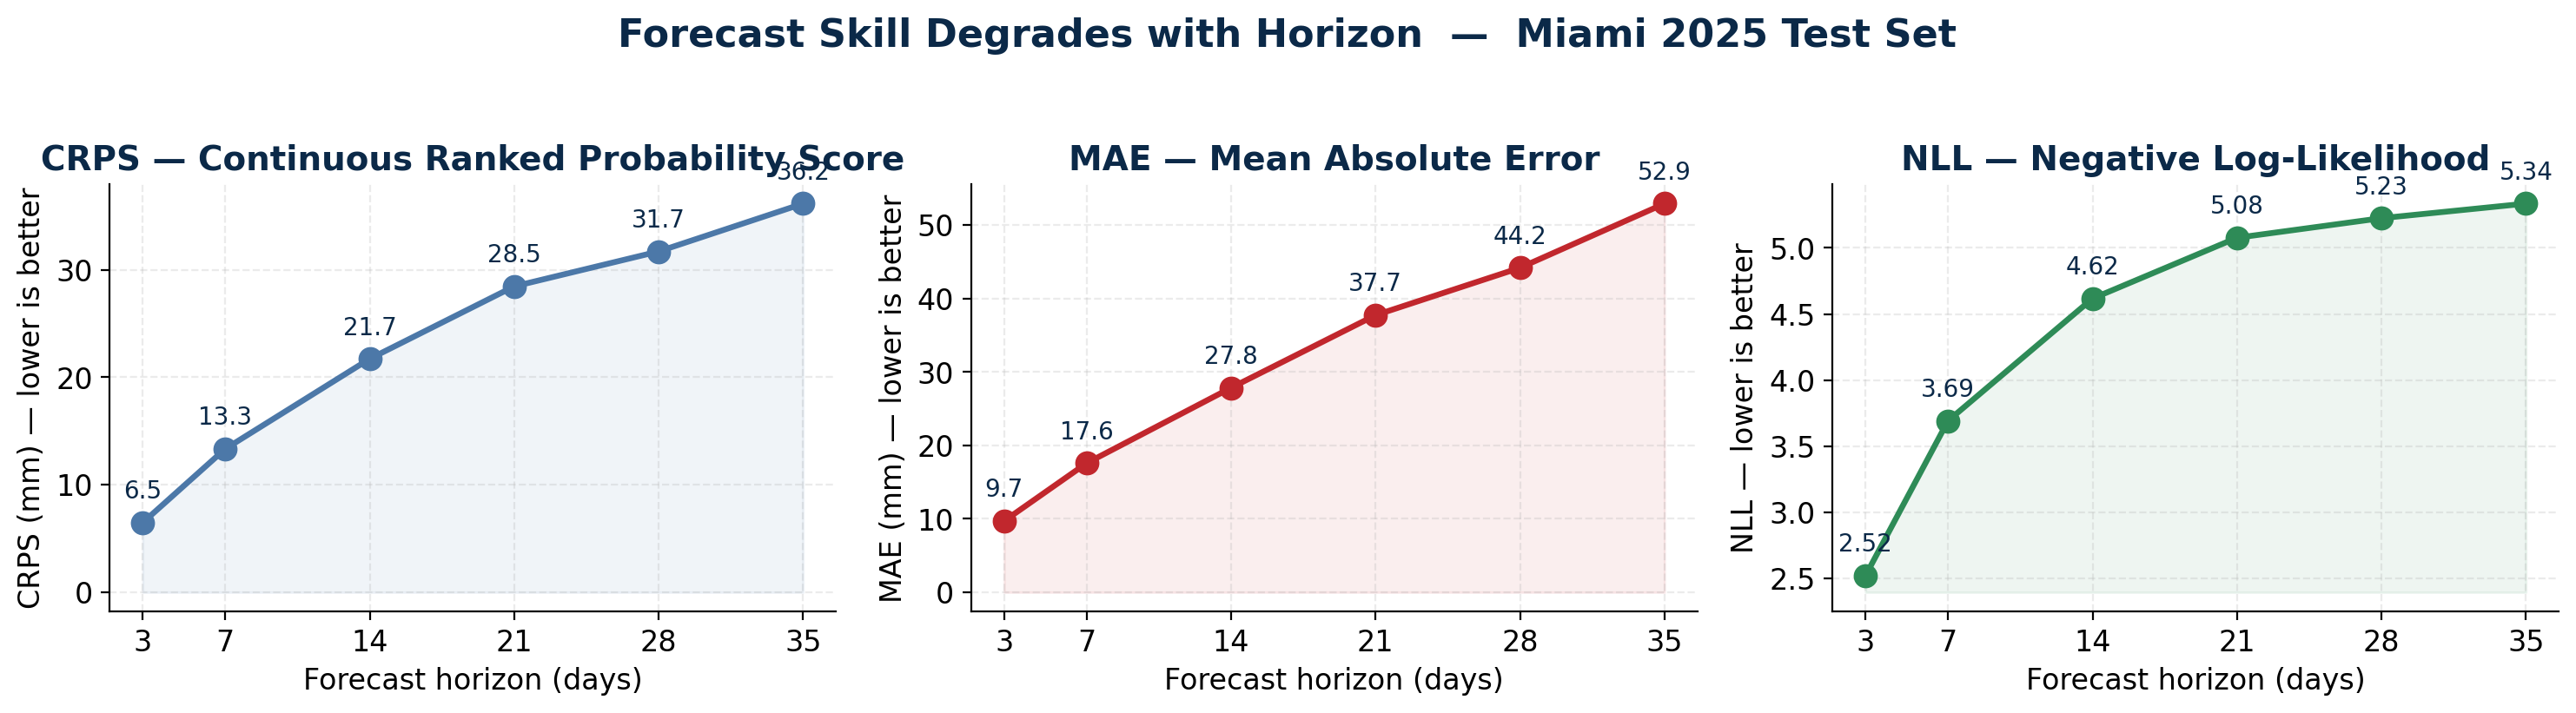
\includegraphics[width=0.85\textwidth]{skill_vs_horizon.png}
    \caption{CRPS skill score (CRPSS) versus climatology baseline by forecast horizon. Positive is better; zero would mean indistinguishable from climatology. The 14-day horizon was the original target; all six are reported here.}
    \label{fig:skill-vs-horizon}
\end{figure}

% ─────────────────────────────────────────────────────────────────────────────
\section{Conclusions and Future Work}

\textbf{Summary.} We built a probabilistic precipitation forecasting system for Miami that fits Gamma distributions to cumulative rainfall over six forecast horizons (3, 7, 14, 21, 28, and 35 days). The pipeline ingests four open data sources, engineers 132 features, trains three distinct distributional ML models, and evaluates them against three classical baselines using strictly proper scoring rules on a held-out 2025 test year.

\textbf{Best method.} \textbf{XGBoost-Gamma} (single XGBoost with the native \texttt{reg:gamma} objective plus MLE shape estimation and post-hoc variance calibration) is our best model, winning on test-set CRPS at five of six horizons. At the original 14-day horizon, it achieves CRPS\,$=$\,21.72\,mm, a 10\% improvement over climatology, 11\% over EMOS-Gamma (the standard NWP post-processing baseline), and 30\% over raw GEFS. The head-to-head total-precipitation comparison in Figure~\ref{fig:head-to-head} backs this up: across all 1{,}460 14-day windows in 2025, XGBoost-Gamma's predicted means sum to within 3.6\% of the observed total, while raw GEFS undershoots by 44.5\%. GAMLSS 2-stage is consistently second and is the most calibrated of the three (its 90\% coverage is closest to nominal). Calibration is now within 5--10 points of nominal across all ML models, compared to the 50+ point miscalibration of the very first prototype reported in the midterm.

\textbf{Practical takeaway.} For point-location precipitation forecasting in a tropical/subtropical climate, a single gradient-boosted Gamma regressor on a rich feature set is the most cost-effective approach we tested. It outperforms two-stage and joint-NLL distributional approaches at every horizon longer than 7 days, while being faster to train and easier to debug.

\textbf{Limitations.} The Gamma distribution has support on $(0, \infty)$, so it cannot put any probability mass at exactly zero. This shows up as a consistent spike near zero in the PIT histograms during the dry season. The validation set is also a single year (2024); a multi-year rolling validation would give more robust calibration but require more computation. Finally, the test set is also a single year (2025), so model rankings could shift in a different climate regime; the 2024--2025 period was warm but not anomalous.

\textbf{Future work.}
\begin{itemize}[leftmargin=1.5em]
    \item \textbf{Zero-inflated distribution.} Replace the Gamma with a censored or shifted Gamma (Scheuerer, 2014), or a hurdle / zero-inflated Gamma mixture so that the model can place explicit mass at zero precipitation. This should fix the dry-season PIT spike.
    \item \textbf{Spatial extension.} The current model is a single-point forecaster. Replicating the same pipeline at every NOAA GHCND station in South Florida and adding spatial features (distance to coast, elevation) would let us produce gridded probabilistic forecasts. This is what neural-network post-processors target.
    \item \textbf{Sub-seasonal-to-seasonal (S2S) extensions.} Push horizons out to 60--90 days using the GEFS ENS extension and ECMWF S2S data. At those horizons, climatology dominates almost entirely, and the question becomes whether ENSO state and MJO phase can produce any useful skill on top.
    \item \textbf{Physical post-processing constraints.} Add side-constraints to ensure that, e.g., a 7-day prediction is always less than a 14-day prediction starting on the same date. The current models do not enforce this; cumulative monotonicity would be a free quality improvement.
\end{itemize}

\textbf{Repository.} All code, processed data instructions, trained model artifacts, the presentation, and this report are organised per the assignment requirements with \texttt{docs/} (presentation + report), \texttt{data/} (with download instructions), \texttt{src/} (training code), and \texttt{scripts/} (data collection, processing, baselines, and visualization helpers).

% ─────────────────────────────────────────────────────────────────────────────
\bibliographystyle{plainnat}
\begin{thebibliography}{12}

\bibitem[Duan et al.(2020)]{duan2020ngboost}
Tony Duan, Anand Avati, Daisy Yi Ding, Khanh~K Thai, Sanjay Basu, Andrew~Y Ng, and Alejandro Schuler.
\newblock {NGBoost}: Natural gradient boosting for probabilistic prediction.
\newblock In \emph{ICML}, 2020.

\bibitem[Gneiting et~al.(2005)]{gneiting2005}
Tilmann Gneiting, Adrian~E. Raftery, Anton~H. Westveld, and Tom Goldman.
\newblock Calibrated probabilistic forecasting using ensemble model output statistics and minimum {CRPS} estimation.
\newblock \emph{Monthly Weather Review}, 133(5):1098--1118, 2005.

\bibitem[Gneiting and Raftery(2007)]{gneiting2007strictly}
Tilmann Gneiting and Adrian~E. Raftery.
\newblock Strictly proper scoring rules, prediction, and estimation.
\newblock \emph{Journal of the American Statistical Association}, 102(477):359--378, 2007.

\bibitem[Gr\"onquist et~al.(2021)]{gronquist2021}
Peter Gr\"onquist, Chengyuan Yao, Tal Ben-Nun, Nikoli Dryden, Peter Dueben, Shigang Li, and Torsten Hoefler.
\newblock Deep learning for post-processing ensemble weather forecasts.
\newblock \emph{Phil. Trans. R. Soc. A}, 379(2194):20200092, 2021.

\bibitem[M\"arz(2022)]{marz2022}
Alexander M\"arz.
\newblock {XGBoostLSS}---An extension of {XGBoost} to probabilistic forecasting.
\newblock \emph{arXiv:2204.06826}, 2022.

\bibitem[Misra et~al.(2011)]{misra2011}
Vasubandhu Misra, Eric Carlson, and others.
\newblock The impact of the wet season on the climate of {S}outh {F}lorida.
\newblock \emph{Journal of Climate}, 24(13):3454--3468, 2011.

\bibitem[Price et~al.(2025)]{price2025graphcast}
Ilan Price, Alvaro Sanchez-Gonzalez, and others.
\newblock Probabilistic weather forecasting with machine learning.
\newblock \emph{Nature}, 2025.

\bibitem[Rasp and Lerch(2018)]{rasp2018}
Stephan Rasp and Sebastian Lerch.
\newblock Neural networks for postprocessing ensemble weather forecasts.
\newblock \emph{Monthly Weather Review}, 146(11):3885--3900, 2018.

\bibitem[Scheuerer(2014)]{scheuerer2014}
Michael Scheuerer.
\newblock Probabilistic quantitative precipitation forecasting using ensemble model output statistics.
\newblock \emph{Quarterly Journal of the Royal Meteorological Society}, 140(680):1086--1096, 2014.

\bibitem[Schlosser et~al.(2019)]{schlosser2019}
Lisa Schlosser, Torsten Hothorn, Reto Stauffer, and Achim Zeileis.
\newblock Distributional regression forests for probabilistic precipitation forecasting in complex terrain.
\newblock \emph{Annals of Applied Statistics}, 13(3):1564--1589, 2019.

\bibitem[Taillardat et~al.(2016)]{taillardat2016}
Maxime Taillardat, Olivier Mestre, Micha\"el Zamo, and Philippe Naveau.
\newblock Calibrated ensemble forecasts using quantile regression forests and ensemble model output statistics.
\newblock \emph{Monthly Weather Review}, 144(6):2375--2393, 2016.

\end{thebibliography}

\end{document}
